\documentclass{article}

%%%%%%%%%%%%%%%%%%%%%%%%%%%%% Using Packages %%%%%%%%%%%%%%%%%%%%%%%%%%%%%%%%%%
\usepackage{float}
\usepackage{geometry}
\usepackage{graphicx}
\usepackage{amssymb}
\usepackage{amsmath}
\usepackage{amsthm}
\usepackage{empheq}
\usepackage{mdframed}
\usepackage{booktabs}
\usepackage{lipsum}
\usepackage{color}
\usepackage{psfrag}
\usepackage{pgfplots}
\usepackage{bm}
\usepackage{csquotes}
\usepackage[spanish]{babel}
\usepackage[style=apa]{biblatex}


%%%%%%%%%%%%%%%%%%%%%%%%%%%%%%%%%%%%%%%%%%%%%%%%%%%%%%%%%%%%%%%%%%%%%%%%%%%%%%%

%%%%%%%%%%%%%%%%%%%%%%%%%% Page Setting %%%%%%%%%%%%%%%%%%%%%%%%%%%%%%%%%%%%%%%
\geometry{letterpaper, margin=2.54cm}
\addbibresource{referencias.bib}
%%%%%%%%%%%%%%%%%%%%%%%%%% Define some useful colors %%%%%%%%%%%%%%%%%%%%%%%%%%
\definecolor{ocre}{RGB}{243,102,25}
\definecolor{mygray}{RGB}{243,243,244}
\definecolor{deepGreen}{RGB}{26,111,0}
\definecolor{shallowGreen}{RGB}{235,255,255}
\definecolor{deepBlue}{RGB}{61,124,222}
\definecolor{shallowBlue}{RGB}{235,249,255}
%%%%%%%%%%%%%%%%%%%%%%%%%%%%%%%%%%%%%%%%%%%%%%%%%%%%%%%%%%%%%%%%%%%%%%%%%%%%%%%

%%%%%%%%%%%%%%%%%%%%%%%%%% Define an orangebox command %%%%%%%%%%%%%%%%%%%%%%%%
\newcommand\orangebox[1]{\fcolorbox{ocre}{mygray}{\hspace{1em}#1\hspace{1em}}}
%%%%%%%%%%%%%%%%%%%%%%%%%%%%%%%%%%%%%%%%%%%%%%%%%%%%%%%%%%%%%%%%%%%%%%%%%%%%%%%

%%%%%%%%%%%%%%%%%%%%%%%%%%%% English Environments %%%%%%%%%%%%%%%%%%%%%%%%%%%%%
\newtheoremstyle{mytheoremstyle}{3pt}{3pt}{\normalfont}{0cm}{\rmfamily\bfseries}{}{1em}{{\color{black}\thmname{#1}~\thmnumber{#2}}\thmnote{\,--\,#3}}
\newtheoremstyle{myproblemstyle}{3pt}{3pt}{\normalfont}{0cm}{\rmfamily\bfseries}{}{1em}{{\color{black}\thmname{#1}~\thmnumber{#2}}\thmnote{\,--\,#3}}
\theoremstyle{mytheoremstyle}
\newmdtheoremenv[linewidth=1pt,backgroundcolor=shallowGreen,linecolor=deepGreen,leftmargin=0pt,innerleftmargin=20pt,innerrightmargin=20pt]{theorem}{Theorem}[section]
\theoremstyle{mytheoremstyle}
\newmdtheoremenv[linewidth=1pt,backgroundcolor=shallowBlue,linecolor=deepBlue,leftmargin=0pt,innerleftmargin=20pt,innerrightmargin=20pt]{definition}{Definition}[section]
\theoremstyle{myproblemstyle}
\newmdtheoremenv[linecolor=black,leftmargin=0pt,innerleftmargin=10pt,innerrightmargin=10pt]{problem}{Problem}[section]
%%%%%%%%%%%%%%%%%%%%%%%%%%%%%%%%%%%%%%%%%%%%%%%%%%%%%%%%%%%%%%%%%%%%%%%%%%%%%%%

%%%%%%%%%%%%%%%%%%%%%%%%%%%%%%% Plotting Settings %%%%%%%%%%%%%%%%%%%%%%%%%%%%%
\usepgfplotslibrary{colorbrewer}
\pgfplotsset{width=8cm,compat=1.9}
%%%%%%%%%%%%%%%%%%%%%%%%%%%%%%%%%%%%%%%%%%%%%%%%%%%%%%%%%%%%%%%%%%%%%%%%%%%%%%%

%%%%%%%%%%%%%%%%%%%%%%%%%%%%%%% Title & Author %%%%%%%%%%%%%%%%%%%%%%%%%%%%%%%%
\title{Taller Resistencia de Materiales}
\author{Gustavo Vergara}
%%%%%%%%%%%%%%%%%%%%%%%%%%%%%%%%%%%%%%%%%%%%%%%%%%%%%%%%%%%%%%%%%%%%%%%%%%%%%%%

\begin{document}

    \begin{titlepage}
\centering


\vspace{3cm}
{\scshape\Huge Trabajo de Resistencia de Materiales \par}
\vspace{5cm}
\textbf\large\scshape{\par}
     \vspace{4cm}
     
{\Large Vergara Pareja Gustavo\\Vergara Germán\\\par}
\vspace{5cm}
{\scshape\Large Robinson Martínez Sandoval \par}
\vspace{0.5cm}
{\scshape\Large Programa de Ingeniería Mecánica \par}
\vspace{1cm}
{\scshape\Large Universidad de Córdoba\par}
\vspace{1cm}
{\Large \today \par}
\end{titlepage}
\newpage
\tableofcontents
\newpage

\section*{Introducción}
\addcontentsline{toc}{section}{Introducción}
Un ascensor o elevador es un dispositivo mecánico que se utiliza para transportar personas o 
cargas entre diferentes niveles de un edificio. En este informe de dinámica, se analizará el 
movimiento de un ascensor que utiliza dos poleas y un dinamo como parte de su diseño mecánico.
El funcionamiento del ascensor se basa en la aplicación de las leyes de Newton y la utilización
 de un sistema de poleas para simular la fuerza necesaria para levantar la carga de un ascensor real.
 \newline 
 El dinamo proporciona la energía necesaria para mover el ascensor, mientras que las poleas
  se utilizan para cambiar la dirección de la fuerza aplicada.
Se responderán preguntas 
como ¿Cómo se diseñó el ascensor?, ¿Con qué materiales se construyó? y ¿Cuál es su finalidad?.
\newline
Para lograr este objetivo, se utilizarán principios de la física y la mecánica para describir
 el movimiento del ascensor y se analizarán las fuerzas involucradas en su funcionamiento. 
 Además, se describirá el diseño mecánico del ascensor, incluyendo los materiales utilizados 
 y las especificaciones técnicas.
 \newpage

\section*{¿Qué se hizo?}
\addcontentsline{toc}{section}{¿Qué se hizo?}

El objetivo de este proyecto fue estudiar el movimiento de un ascensor o elevador y realizar cálculos empíricos
 de su velocidad, aceleración y distancia recorrida. En la práctica, se construyó una maqueta de ascensor a pequeña escala y se realizaron experimentos para medir
 \begin{itemize}
    \item El tiempo que tarda en subir y bajar entre pisos.
    \item Demostrar conceptos de dinámica como la aceleración, la velocidad y la gravedad que afectan el movimiento de un ascensor real.
 \end{itemize}

\section*{Materiales y métodos}
\addcontentsline{toc}{section}{Materiales y métodos}
Los materiales utilizados para el desarrollo de este eleveador fueron:

\begin{itemize}
  \item 1 dinamo
  \item 2 cajas pequeñas (40gc/u)
  \item 1 caja grande
  \item 1 interruptor
  \item 2 minipoleas
  \item 2 gotas mágicas
  \item 1 batería 9V
\end{itemize}
\newpage
\section*{Contenido y Resultados}
\addcontentsline{toc}{section}{Contenido y Resultados}
Para el desarrollo de este proyecto, realizamos varios planos antes de construir:
\begin{figure}[H]
\centering
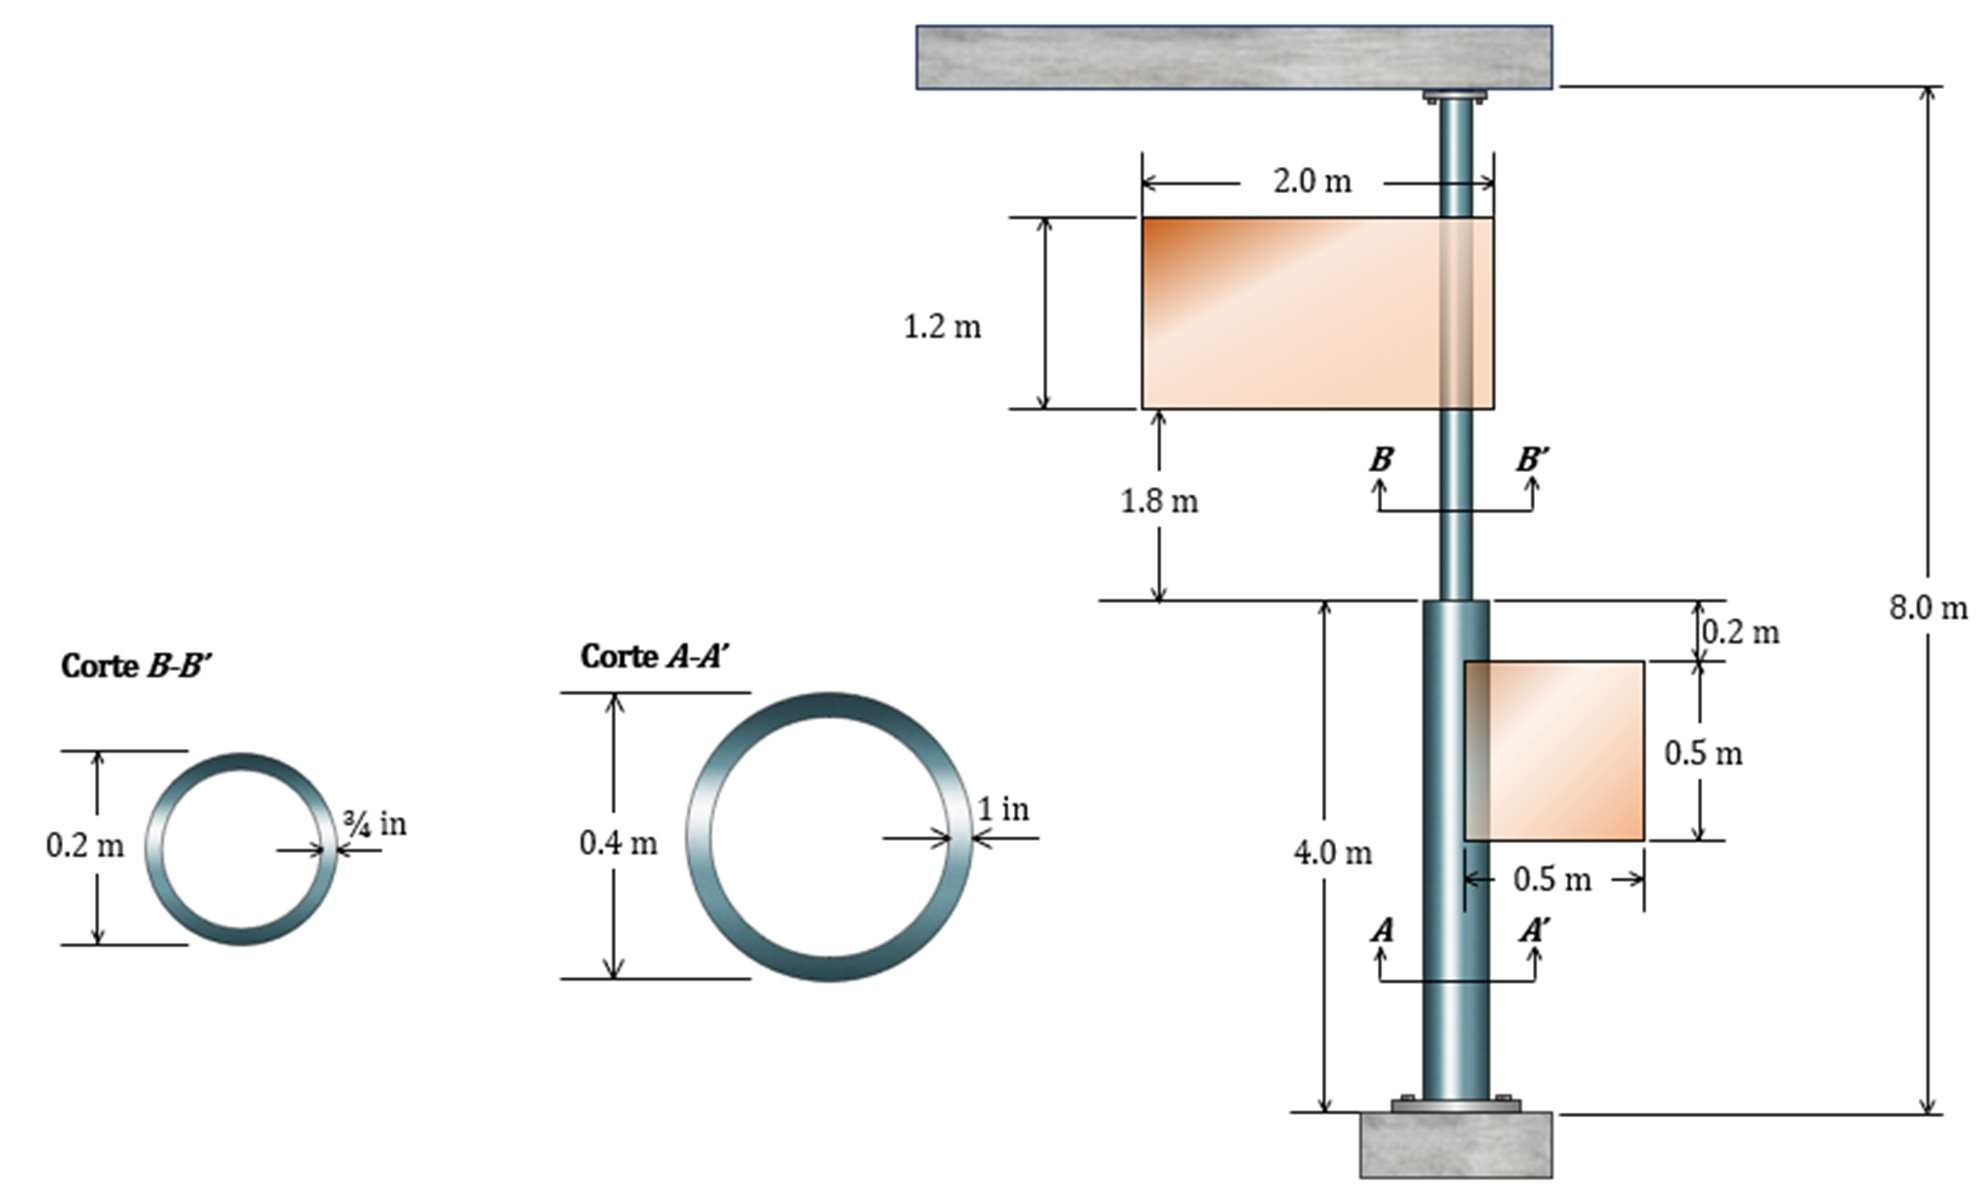
\includegraphics[width=0.5\textwidth]{Picture1.jpg}
\caption{Plano antes de construir}
\label{fig:imagen}
\end{figure}
\begin{itemize}
\item Luego de esto, pasamos a crear el elevador:
\end{itemize}
\begin{figure}[H]
\centering
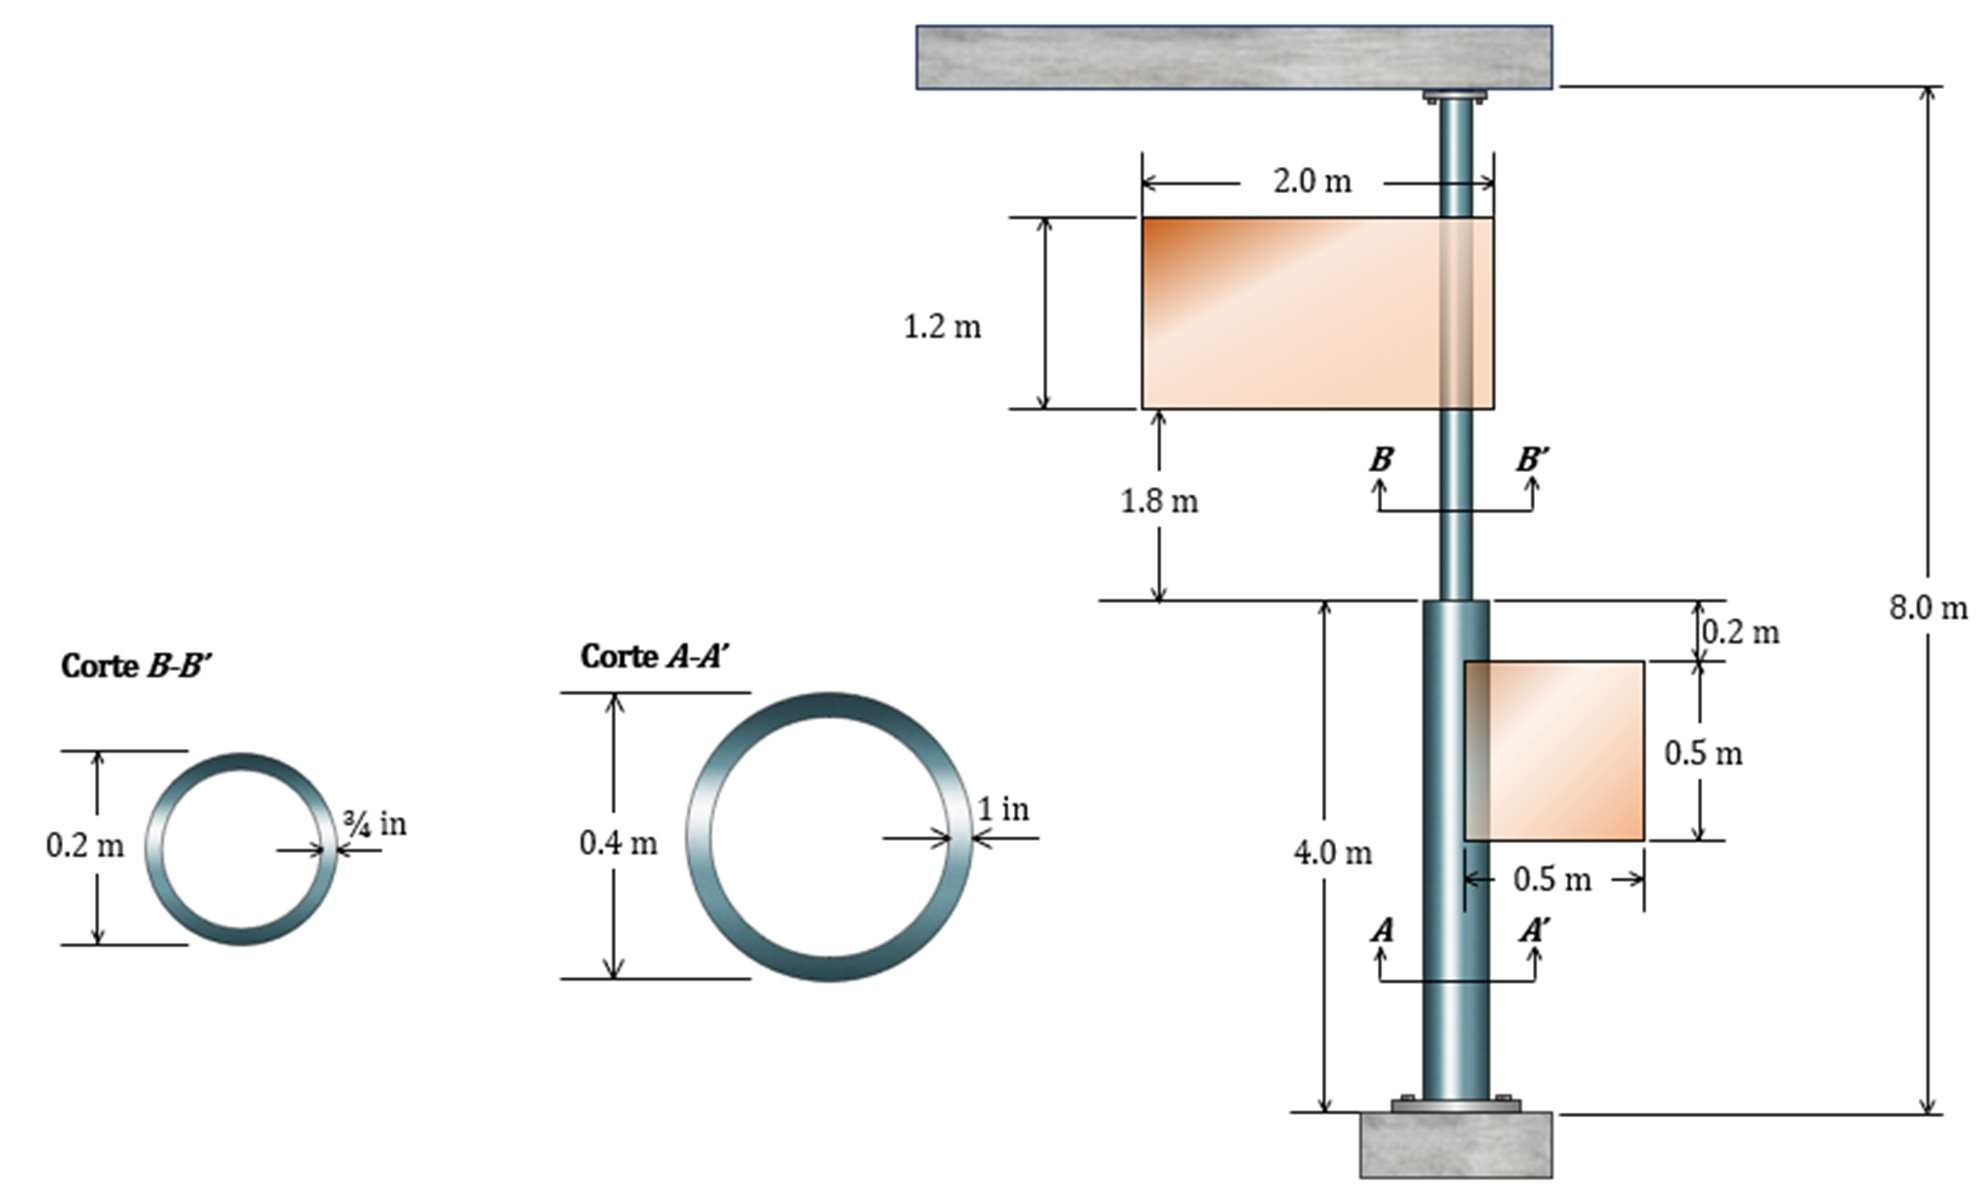
\includegraphics[width=0.5\textwidth]{Picture1.jpg}
\caption{Elevador construido}
\label{fig:imagen1}
\end{figure}
\begin{itemize}
\item Para su versión final generamos un plano en SolidWorks.
\end{itemize}
\begin{figure}[H]
    \centering
    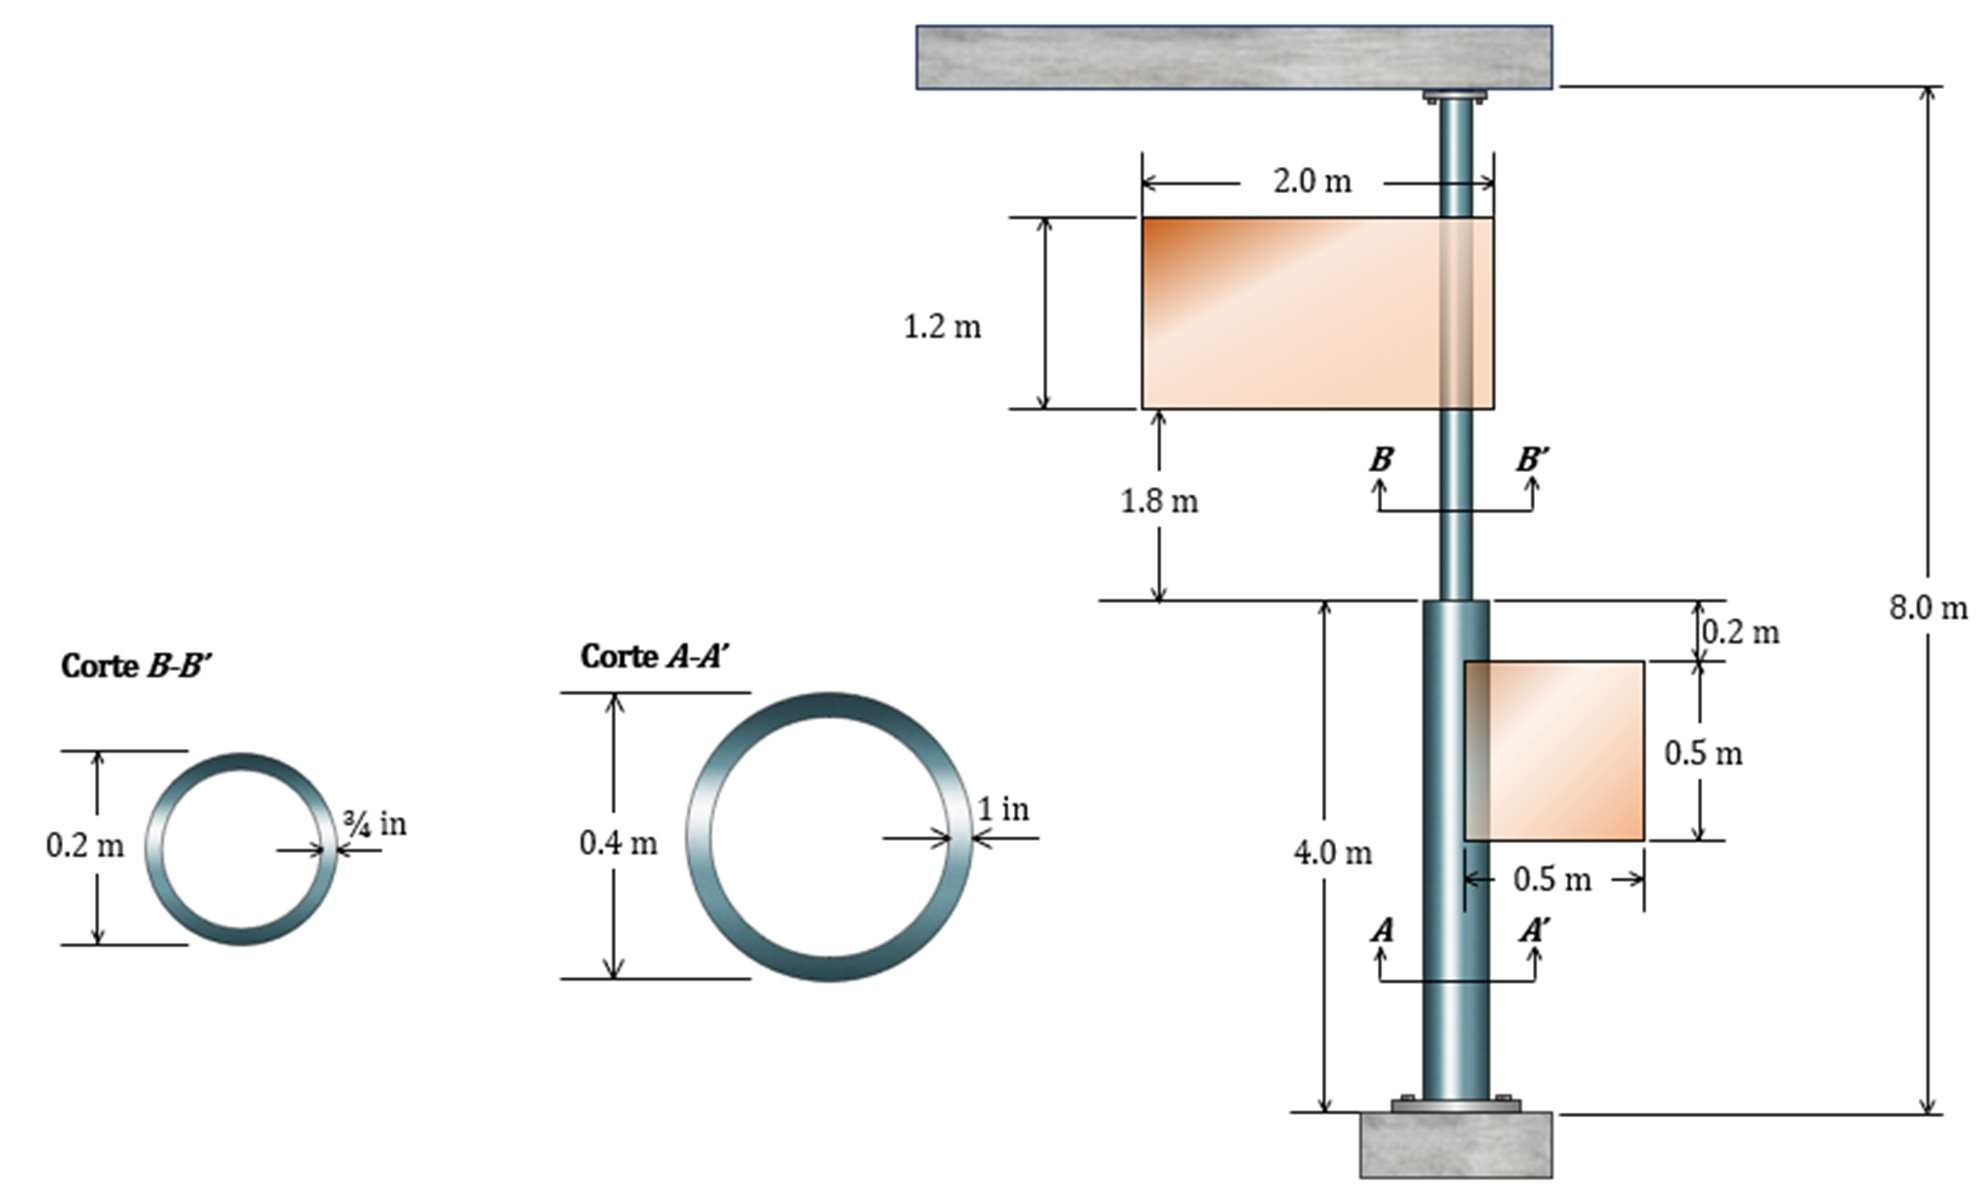
\includegraphics[width=0.8\textwidth]{Picture1.jpg}
    \caption{Elevador en SolidWorks}
    \label{fig:imagen2}
    \end{figure}
    \begin{itemize}
    \item Para el análisis dinámico se debe simplificar la estructura con el fin de poder analizarla y aproximar lo ocurrido.
    \end{itemize}
    \begin{figure}[H]
    \centering
    
    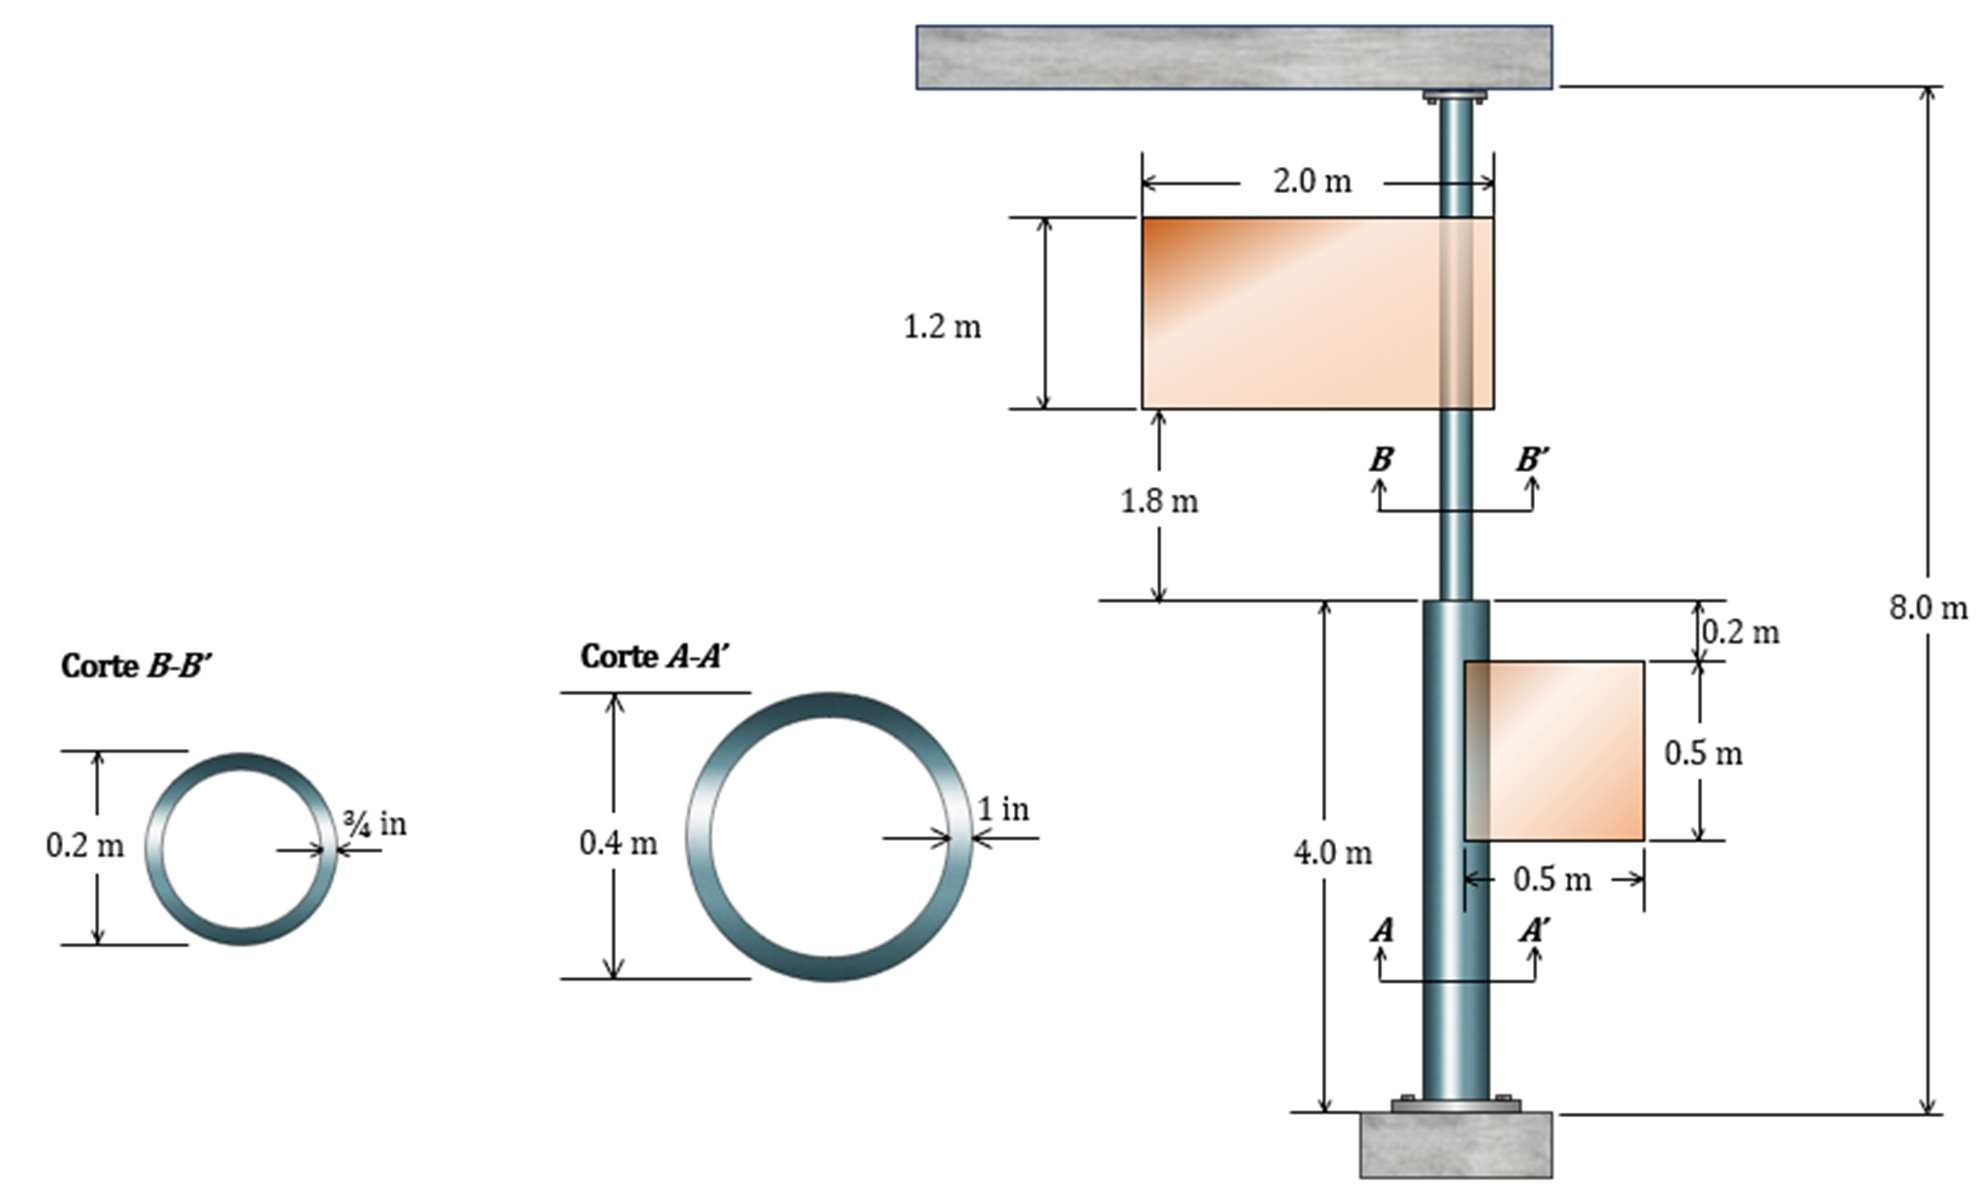
\includegraphics[width=0.8\textwidth]{Picture1.jpg}
    \caption{Elevador listo para analizar en SolidWorks}
    \label{fig:imagen3}
    \end{figure}
    \newpage
    Para este ascensor, los calculos se simplifican mucho, ya que ambas cabinas se mueven a la misma velocidad
    aportada por el motor. La diferencia es que es en sentidos contrarios. Para el análisis dinámico entonces calcularemos:

    \begin{itemize}
        \item Velocidad
     \newline
        $$v=\frac{y}{t}=\frac{0.1m}{1s}=10cm/s$$
        \item Aceleracion
        \newline
        La aceleración de las cabinas sera igual a 0, ya que por la primera Ley de Newton, estos cuerpos
        estan bajo velocidad constante. 
        \item Tensión 
        \newline
        Podemos calcular fuerza de tensión en los cables que sostienen las cabinas. Para hacer esto, podemos usar la segunda ley de Newton, que establece que la fuerza neta sobre un objeto es igual a su masa multiplicada por su aceleración. En este caso, la aceleración de las cabinas es cero, por lo que la fuerza neta es cero. Por lo tanto, la suma de las fuerzas en cada cabina debe ser igual a cero. Podemos escribir esto como:
        \newline
       $$F_{T}-\left ( m_{1}*g \right )-\left ( m_{2}*g \right )=0$$
        $$F_{T}=\left ( 0.04kg*9.81\frac{m}{{s}^2} \right )+\left ( 0.04kg*9.81\frac{m}{{s}^2} \right )=0.8N$$
        \item Potencia
        $$W=2T\cdot v=\left ( 0.8N \right )\left ( 0.1m/s \right )=0.08W$$
        \item Velocidad angular del eje
        Podemos calcular la velocidad angular del eje utilizando la fórmula:
        \newline
        $$w = v/r$$
        $$w =\left ( 0.1m/s \right )/\left ( 0.02m \right )=5 rad/s$$
      \end{itemize}


    \section*{Conclusiones}
    \addcontentsline{toc}{section}{Conclusiones}
    En conclusión, se logró estudiar el movimiento de un ascensor o elevador y realizar cálculos empíricos de su velocidad, aceleración y distancia recorrida. Se construyó una maqueta de ascensor a pequeña escala y se realizaron experimentos para medir el tiempo que tarda en subir y bajar entre pisos y demostrar conceptos de dinámica como la aceleración, la velocidad y la gravedad que afectan el movimiento de un ascensor real. Los cálculos se simplificaron mucho, ya que ambas cabinas se mueven a la misma velocidad aportada por el motor. La diferencia es que es en sentidos contrarios. Se calculó la velocidad, la aceleración, la fuerza de tensión en los cables que sostienen las cabinas, la potencia y la velocidad angular del eje.
    
    \newpage
   
    \section*{Bibliografía}
    \printbibliography 
\end{document}